\documentclass[conference]{IEEEtran}
\IEEEoverridecommandlockouts
% The preceding line is only needed to identify funding in the first footnote.
% If that is unneeded, please comment it out.
%\usepackage[backend=bibtex,style=verbose-trad2]{biblatex}

\usepackage{adjustbox}
\usepackage{algorithmic}
\usepackage{amsmath,amssymb,amsfonts}
%\usepackage[backend=bibtex,style=ieee]{biblatex}
%\usepackage{bookmark}
\usepackage{tabularx,array}
\usepackage{booktabs}
\usepackage{caption}
\usepackage{cite}
\usepackage{color}
\usepackage[inline]{enumitem}
\usepackage{float}
\usepackage[T1]{fontenc}
%\usepackage{fontspec}
\usepackage{footnote}
\usepackage{graphicx}
\usepackage[colorlinks=true,citecolor=blue]{hyperref}
\usepackage{inputenc}[utf8]
\usepackage{listings}
\usepackage{textcomp}
\usepackage[flushleft]{threeparttable}
\usepackage{subcaption}
\usepackage{xcolor}

\title{QEMU Computation Storage Devices%\\
%{\footnotesize \textsuperscript{*}Note: Sub-titles are not captured in Xplore 
% and should not be used}
%\thanks{Identify applicable funding agency here. If none, delete this.}
}

\pagenumbering{arabic}
\pagestyle{plain}

% Ensure decimal numbering in table  of contents
\renewcommand{\thesection}{\arabic{section}}
\renewcommand{\thesubsection}{\arabic{section}.\arabic{subsection}}
\renewcommand{\thesubsubsection}{\arabic{section}.\arabic{subsection}.\arabic{subsubsection}}

% ensure decimal numbering for sub sections
\makeatletter
\renewcommand{\@seccntformat}[1]{\csname the#1\endcsname.\quad}
\makeatother

% ------------------------------------------------------------------------%
% Proper Python Syntax Highlighting                                       %
% Author: redmode
% https://tex.stackexchange.com/questions/83882/how-to-highlight-python   %
% -syntax-in-latex-listings-lstinputlistings-command#83883                %
% ----------------------------------------------------------------------- %

% Default fixed font does not support bold face
\DeclareFixedFont{\ttb}{T1}{txtt}{bx}{n}{8} % for bold
\DeclareFixedFont{\ttm}{T1}{txtt}{m}{n}{8}  % for normal

% Custom colors
\definecolor{deepblue}{rgb}{0,0,0.5}
\definecolor{deepred}{rgb}{0.6,0,0}
\definecolor{deepgreen}{rgb}{0,0.5,0}

% Python style for highlighting
\newcommand\pythonstyle{
	\lstset{
		language=Python,
		basicstyle=\ttm,
		showstringspaces=false,
		tabsize=4,
		aboveskip=0.2cm,
		belowskip=0.2cm,
		otherkeywords={self},             % Add keywords here
		keywordstyle=\ttb\color{deepblue},
		emph={MyClass,__init__},          % Custom highlighting
		emphstyle=\ttb\color{deepred},    % Custom highlighting style
		stringstyle=\color{deepgreen},
		frame=tb,                          % Any extra options here
		prebreak=\textbackslash,
		linewidth=8.85cm,
		breaklines=true,
	}
}

% Python environment
\lstnewenvironment{python}[1][] {
	\pythonstyle\lstset{#1}
}{}

% Python for inline
\newcommand\pythoninline[1]{{\pythonstyle\lstinline!#1!}}

% Python for external file
\newcommand\pythonexternal[2][]{{\pythonstyle\lstinputlisting[#1]{#2}}}

% ----------------------------------------------------------------------- %

% Bash style for highlighting
\newcommand\bashstyle{
	\lstset{
		language=Bash,
		basicstyle=\ttm,
		showstringspaces=false,
		tabsize=2,
		%commentstyle=itshape,
		aboveskip=0.2cm,
		belowskip=0.2cm,
		prebreak=\textbackslash,
		extendedchars=true,
		mathescape=false,
		% literate= {\$}{{\textcolor{blue}{\$}}}1 {&}{{\textcolor{blue}{\&}}}1 {/n}{{\textcolor{green}{\textbackslash n}}}1,
		linewidth=8.85cm,
		breaklines=true
	}
}

% Bash environment
\lstnewenvironment{bash}[1][] {
	\bashstyle\lstset{#1}
}{}

% Bash for inline
\newcommand\bashinline[1]{{\bashstyle\lstinline!#1!}}

% Bash for external file
\newcommand\bashexternal[2][]{{\bashstyle\lstinputlisting[#1]{#2}}}


% Python style for highlighting
\newcommand\cstyle{
	\lstset{
		language=c,
		basicstyle=\ttm,
		showstringspaces=false,
		tabsize=4,
		aboveskip=0.2cm,
		belowskip=0.2cm,
		otherkeywords={self},             % Add keywords here
		keywordstyle=\ttb\color{deepblue},
		emph={MyClass,__init__},          % Custom highlighting
		emphstyle=\ttb\color{deepred},    % Custom highlighting style
		stringstyle=\color{deepgreen},
		frame=tb,                          % Any extra options here
		prebreak=\textbackslash,
		linewidth=8.85cm,
		breaklines=true,
	}
}

% Python environment
\lstnewenvironment{clist}[1][] {
	\cstyle\lstset{#1}
}{}

% Python for inline
\newcommand\cinline[1]{{\cstyle\lstinline!#1!}}

% Python for external file
\newcommand\cexternal[2][]{{\cstyle\lstinputlisting[#1]{#2}}}

% ----------------------------------------------------------------------- %

\begin{document}

\begin{titlepage}
\begingroup
\centering
{\LARGE\bfseries QEMU Computational Storage Devices}

\vspace{1cm}

{\Large Vrije Universiteit (VU)}

\vspace{0.5cm}

{Corne Kenneth Lukken}

{\textit{Department of Computer Science} \\
Amsterdam, Netherlands \\
info@dantalion.nl}

\vspace{4.0cm}

%\begin{figure}[H]
%	\centering
%	\includegraphics[width=0.7\textwidth]{resources/images/cover-image.png}
%	\captionsetup{justification=centering}
%	\caption{This is the cover image}
%\end{figure}

\vfill
\endgroup
\hfill
\begin{minipage}{0.3\textwidth}
\begin{flushright}
	
\includegraphics[width=\textwidth]{resources/images/vu-logo.png}
\end{flushright}
\end{minipage}
\end{titlepage}

\clearpage
\onecolumn

% Ensure black link color in table of contents
\hypersetup{
	linkcolor=black
}

\renewcommand{\contentsname}{CONTENTS}
\tableofcontents{}

\hypersetup{
	linkcolor=blue
}

\twocolumn

\addcontentsline{toc}{section}{\protect\numberline{}INTRODUCTION}
\section*{INTRODUCTION}

Recently pieces of literature have been presented about Zones Namespace (ZNS)
SSDs. These cover a variety of topics such as migrating from Open-Channel
SSDs to Zoned Namespaces\cite{bjorling2019open}. Other literature addresses
some of the  functionality these ZNS SSDs introduce\cite{bjorling2020zone}.
Finally, some works evaluate host-based SSD features such as flash management
and  garbage collection when implemented using ZNS SSDs\cite{254268,9188086}.

In this work the use of ZNS SSDs as Computational Storage Device (CSD) will be
investigated. However, this requires the availability of ZNS SSD devices.
Currently, the availability of physical ZNS SSDs is problematic, this is
likely  due to the NVMe Zoned Namespace technical proposal only being ratified
recently\cite{zns-nvme-ratified}.

This NVMe Zoned Namespace command set specification is what enables ZNS SSDs to
exist\cite{nvme-zns}. Luckily, the functionality of this NVMe command set is
already enabled in QEMU. This allows the development of technologies utilizing
ZNS SSDs in a virtualized environment.

Several online resources exist explaining how this functionality was enabled in
QEMU\cite{nvme-qemu-1,nvme-qemu-2} as well as resources on general information
about ZNS SSDs\cite{zns-info}.

This work focuses on documenting the steps necessary to implement CSDs
utilizing ZNS SSDs with QEMU. The emphasis is on describing existing
technologies and how to combine these in a working prototype.

The overall structure of this work is as follows. Introduce several project
dependencies and how to configure these, describe development and debugging
methodologies and how these can be configured by the CMake project accompanying
this work, describe the existing technologies that are used in the final
prototype, define design requirements and the final implemented design as well
as limitations, mention alternative technologies and why they are not used in
the prototype, finally, describe future work and open questions that arise from
this design.

\section{Setting up Dependencenies}

\subsection{Enabling ZNS SSD in QEMU}

The first step is getting an install of QEMU that supports ZNS SSDs. It turned
out that at the time of writing\footnotemark[1] this feature was not actually
upstream yet. By tracing patches a public repository containing these patches
is found. This can subsequently be included as git submodule allowing for a
CMake project to automatically download and install it. The remainder of this
section describes parameters to configure ZNS SSDs in QEMU. However, first the
use and features of git submodules are briefly explained.

\footnotetext[1]{Time of writing is $10^{th}$ of February 2021.}

\subsection{Git Submodules}

Throughout this work git submodules are used extensively, these allow for easy
integration of dependencies into a target project. A submodule can be added by
executing\bashinline{git submodule add REPO_URL.git PATH}. The subsequent
module is than added to the \textit{.gitmodules} file. As an example the
contents of the file for this project is shown in
figure \ref{fig:example-gitmodules}. Git will keep track of the commit each of
these  submodules are checked out on as long as that commit can be found on the
remote referenced in the \textit{.gitmodules} file. Git does not automatically
download  submodules upon cloning a repository. Instead, it offers several
commands to  interact with submodules. The most important of these commands
being\bashinline{git submodule update --init}. If desired the submodules of
submodules can also be initialized recursively by adding\bashinline{--recursive}
to this command.

\begin{center}
	\begin{figure}[H]
		\bashexternal{resources/bash/gitmodules.sh}
		\captionsetup{justification=centering}
		\caption{Contents of \textit{.gitmodules} file for this project.}
		\label{fig:example-gitmodules}
	\end{figure}
\end{center}

\subsubsection{ZNS SSD Configuration}

In parallel with the development of ZNS SSD patches for QEMU are patches that
separate the NVMe devices. These patches allow fine grained control over the
hierarchy of these devices. Among these devices are so called
\textit{subsystems} and \textit{namespaces}. These subsystems effectively allow
namespaces to be shared by multiple NVMe devices. While, namespaces are what
enables ZNS SSDs. The first example shown in
figure \ref{fig:example-nvme-subsystems} illustrates sharing a namespace with
multiple  devices through a subsystem. These examples shown are incomplete, a
complete  example is shown at the end of this section.

\begin{center}
	\begin{figure}[H]
		\bashexternal{resources/bash/nvme-subsystem.sh}
		\captionsetup{justification=centering}
		\caption{Example sharing a single NVMe namespace with two NVMe devices.}
		\label{fig:example-nvme-subsystems}
	\end{figure}
\end{center}

Many types of devices expose important configuration parameters including
NVMe devices. While it would serve little purpose iterating all parameters here,
it is important to know how these can be queried. By
executing\bashinline{qemu-system-x86_64 -device nvme-ns,?} , all parameters for
a NVMe namespace are shown. The type of device can be replaced with any other
device, although some do not expose any configuration parameters.

This final example, shown in figure \ref{fig:qemu-launch}, is a complete set of
parameters to boot QEMU and expose a ZNS SSD. Coincidentally, it is the
command used throughout this project.

Important parameters include \textit{zoned=true} which configures the namespace
to be zoned as well as \textit{bus=nvme2} to link the namespace to the NVMe
device. Additionally, \textit{max\_open} and \textit{max\_active} configure the
maximum number of open and active zones, respectively. Importantly,
\textit{append\_size}, \textit{zone\_size} and \textit{zone\_capacity} must all
be at least 4096.

\begin{center}
	\begin{figure}[H]
		\bashexternal{resources/bash/qemu-launch.sh}
		\captionsetup{justification=centering}
		\caption{Command used to launch QEMU in this project.}
		\label{fig:qemu-launch}
	\end{figure}
\end{center}

\subsection{SPDK}

Another problematic dependency of this project is SPDK. This
framework\footnotemark[2] serves as user space driver for storage devices,
including NVMe. All though, there is abundant documentation for SPDK it is
not trivial to make sense of it all. Important to know is that SPDK itself has
several dependencies it requires to operate. These include DPDK and isa-l among
others.

\footnotetext[2]{The term library would be misleading given the scale of SPDK.}

\subsubsection{Static vs Dynamic Linking}

Initially, the CMake project was configured to statically compile and install
SPDK, however, this resulted in erratic runtime behavior. When instead compiling
SPDK as shared library this behavior was resolved. A bug report has been
submitted to the SPDK repository describing the issue in more
details\cite{spdk-bug}. The likely cause of this behavior is that runtime checks
ensure the availability of a certain set of features, the library to enable
PCI-e is likely missing from the statically linked set. Since the shared
library links to all other shared libraries of SPDK, the library to enable
PCI-e is automatically linked as well. If this is indeed the case, a good
suggestion would be to improve the documentation to show which libraries enable
which drivers and interfaces. Alteratively, the targets could be linked against
all static libraries.

The authors of SPDK are very helpful and provided clear insights into why
static compilation is not working when used this way. Their framework relies on
constructor functions to register NVMe transport types. These are only exported
if the static archive is linked using\bashinline{-Wl,--whole-archive}. The
documentation has been improved to better indicate these linkage
requirements\cite{spdk-documentation-patch}.

\subsubsection{Periodic Setup}

Before SPDK can be used the NVMe devices have to be assigned to the correct
driver as well as requiring that several hugepages are setup. The SPDK source
provides a simple shell script that allows to perform these actions easily.
These  changes are restored upon reboot, meaning the script has to be run again
after each reboot. This setup can be performed by
executing\bashinline{sudo HUGEMEM=512 /home/arch/qemu-csd/dependencies/spdk/scripts/setup.sh},
Alternatively, a systemd service can be created to automatically perform this
setup upon boot. An example of such a systemd service file is shown in
figure \ref{fig:spdk-service}.

\begin{center}
	\begin{figure}[H]
		\bashexternal{resources/bash/spdk.service}
		\captionsetup{justification=centering}
		\caption{Systemd service file to setup SPDK requirements upon boot.}
		\label{fig:spdk-service}
	\end{figure}
\end{center}

Several locations can be chosen to install a systemd service file, all of which
are valid. The most commonly used onces are listed here \begin{enumerate*}
\item \textit{/etc/systemd/system/} \item \textit{/usr/lib/systemd/system/}
\end{enumerate*}. The use of \textit{system} subdirectories is preferred as it
will involve a service that runs without using \textit{User=}. Essentially, this
means that environment variables such as \textit{\$HOME} will not be configured.
After creating a new systemd service file in an appropriate directory, the
daemon must be reloaded for it to be listed. This can be done by
executing\bashinline{sudo systemctl daemon-reload}. The usual \textit{enable}
and \textit{start} commands can now be used to configure the service to start
on boot and start it manually, respectively. Take into account that regular
tools relying on the \textit{nvme} kernel module can no longer be used if this
procedure is performed on startup. Some of these include \textit{nvme-cli} or
\textit{blkzone} as well as the block device disappearing from \textit{/dev}.
An overview of which tools are influenced is shown in figure
\ref{fig:spdk-landscape}.

To test that this setup has been performed correctly the examples from the spdk
directory can be used. The identify example should report an output comparable
to the example shown in figure \ref{fig:spdk-identify}. This identify binary can
be found in
\textit{/home/arch/qemu-csd/dependencies/spdk/build/examples/identify}, note
that it needs to be run with sudo privileges and \textit{\$LD\_LIBRARY\_PATH}
configured. If the build environment is activated the \textit{ld-sudo} alias can
be used for this.

\begin{center}
	\begin{figure}[H]
		\bashexternal{resources/bash/identify-output.sh}
		\captionsetup{justification=centering}
		\caption{Partial output of SPDK identify binary when running QEMU with default
			parameters.}
		\label{fig:spdk-identify}
	\end{figure}
\end{center}

\section{Development \& Debugging}

Anyone is free to use any developments tools they would like but several are
more tightly integrated into this project. These primarily are Clion \& vscode.
Initially, a section to describe the use of development tools might seem trivial
or redundant. However, fast effective iteration cycles are essential for quickly
developing projects, such as those in a research settings. The effective use of
development tools is essential for this fast iteration.

\subsection{Clion}

Since Clion understands CMake, it is able to find the headers of used
dependencies. The default key binding for this is \textit{ctrl+b}. This code
inspection also works across different pars of qemu-csd. From CMake it is also
able to deduce any compilation targets. Different profiles can be created to
adjust any configuration parameters of the project, such as
\textit{-DENALBE\_PLAYGROUND} or \textit{-DIS\_DEPLOYED}. These profiles can be
found  under \textit{Settings -> Build, Execution, Deployment -> CMake -> Profiles}.

In addition to profiles, CMake also maintains a set of toolchains. By default
a toolchain is included that uses a bundled version of CMake. This bundled
version might be insufficient to run this CMake project. New toolchains can be
configured under \textit{Settings -> Build, Execution, Deployment -> Toolchains}.
Subsequently, toolchains can be assigned to profiles in the CMake profiles menu.

Some targets, such as \textit{play-spdk}, might require root privileges to run.
Any target can be configured to run with root privileges. Simply press on the
target selection bar in the top right corner and select
\textit{Edit configurations}. For each of the binary targets a toggle witht
\textit{Run with root privileges} should be visible.

One of the limitations of Clion is that it can only debug targets found through
CMake. This prohibits remote debugging such as required when debugging binaries
running inside QEMU. For this type of debugging vscode can be used instead.

\subsection{Vscode}

Unlike Clion, vscode does not automatically detect any possible debugging
targets based on project files in the directory. Instead it manually requires to
configure a \textit{launch.json} file in the .vscode directory. This allows this
project to pre-configure any targets that can be debugged in QEMU as well as
providing an example for possible future extensions.

The \textit{SSH attach play-spdk} target is configured to login over SSH, run
the bootstrap commands and start a gdb session. The information retrieved from
gdb will than be used to update the GUI like in many other IDEs. This
configuration relies on a clever trick that the \textit{cwd} + \textit{target}
path on the host correspond to the \textit{ssh: cwd} + \textit{target} path on
the guest. This allows for a translation of paths between host and guest so
that vscode can  still find the corresponding source files. This behavior is
very similar if not identical to gdb \textit{set substitute-path}.

\subsection{Gdbserver}

As an alternative to GUI based debuggers, a combination of gdb \& gdbserver can
be used as well. On QEMU start the gdbserver on port 2000 for
instance\bashinline{gdbserver localhost:2000 playground/play-spdk}. While on the
host gdb would be launched. Within gdb the commands shown in
figure \ref{fig:gdb-qemu} would be executed to setup the debugging. The second
parameter of \textit{substitute-path} needs to match the absolute path to the
root of the qemu-csd directory.

\begin{center}
	\begin{figure}[H]
		\bashexternal{resources/bash/gdb-qemu.sh}
		\captionsetup{justification=centering}
		\caption{Commands to configure gdb for debugging when binary is run
			within QEMU.}
		\label{fig:gdb-qemu}
	\end{figure}
\end{center}

\subsection{Stacktraces}

Stacktraces can be very informative when debugging runtime exceptions such as
segmentation faults. When CMake is configured for a Debug build type all binary
targets will be linked against backward-cpp. This library enables extensive
stacktraces which include line numbers. An example of how these stracktraces can
be displayed manually can be found in
\textit{playground/backward/playground-backward.cxx}. To enable backward on a
target in CMake the command \textit{qemucsd\_target\_postprocess(\$TARGET)} must
be  called with the name of the target as argument.

\subsection{CMake build types}

Backward can be disabled by configuring CMake with
\textit{-DCMAKE\_BUILD\_TYPE=Release}. This will also compile the target to use
machine specific optimizations such as relying on instruction set extensions
like AVX512. The release build type is not compatible with code coverage or with
address sanitizer.

\subsection{Address sanitization}

Sometimes stacktraces are not enough. Memory errors that take several iterations
or events before they lead to failure or non-determinsm in when an error occurs
might make it difficult to find the root cause of a problem. For these cases the
CMake project is configurable with an option that will enable address
sanitization. Address sanitization will halt the execution of the running binary
as soon as a single memory error occurs. These runtime detections of memory
errors will not catch all but most errors. To enable this feature the parameter
\textit{-DENABLE\_LEAK\_TESTS=on} must be set to on.

\section{Technology Backgrounds}

This section highlights how different technologies are realised. This ranges
from insights about specifications, libraries, frameworks and drivers. Typically
this includes figures about landscapes that provide an overview of how these
technologies tie together. However, it does not include any examples or
recommendation on how all these technologies together can be used to enable
CSDs in QEMU. The specific case of enabling CSDs in QEMU will be discussed in
details later.

\subsection{SPDK}

SPDK is a technology that allows interfacing with storage devices from userspace.
In addition, it recently has gotten support for ZNS SSDs. The technology
requires to assign one of several drivers to storage devices as well as setting
up hugepages. SPDK can also be used without root permissions if the
permissions on devices and hugepages have been properly configured. Because
SPDK relies on reassigning device drivers, several tools will become
unavailable. Some of the tools involved are shown in figure
\ref{fig:spdk-landscape}. The advantage of SPDK is that it allows for an
interface without file or block layer abstractions.

\begin{center}
	\begin{figure}[H]
		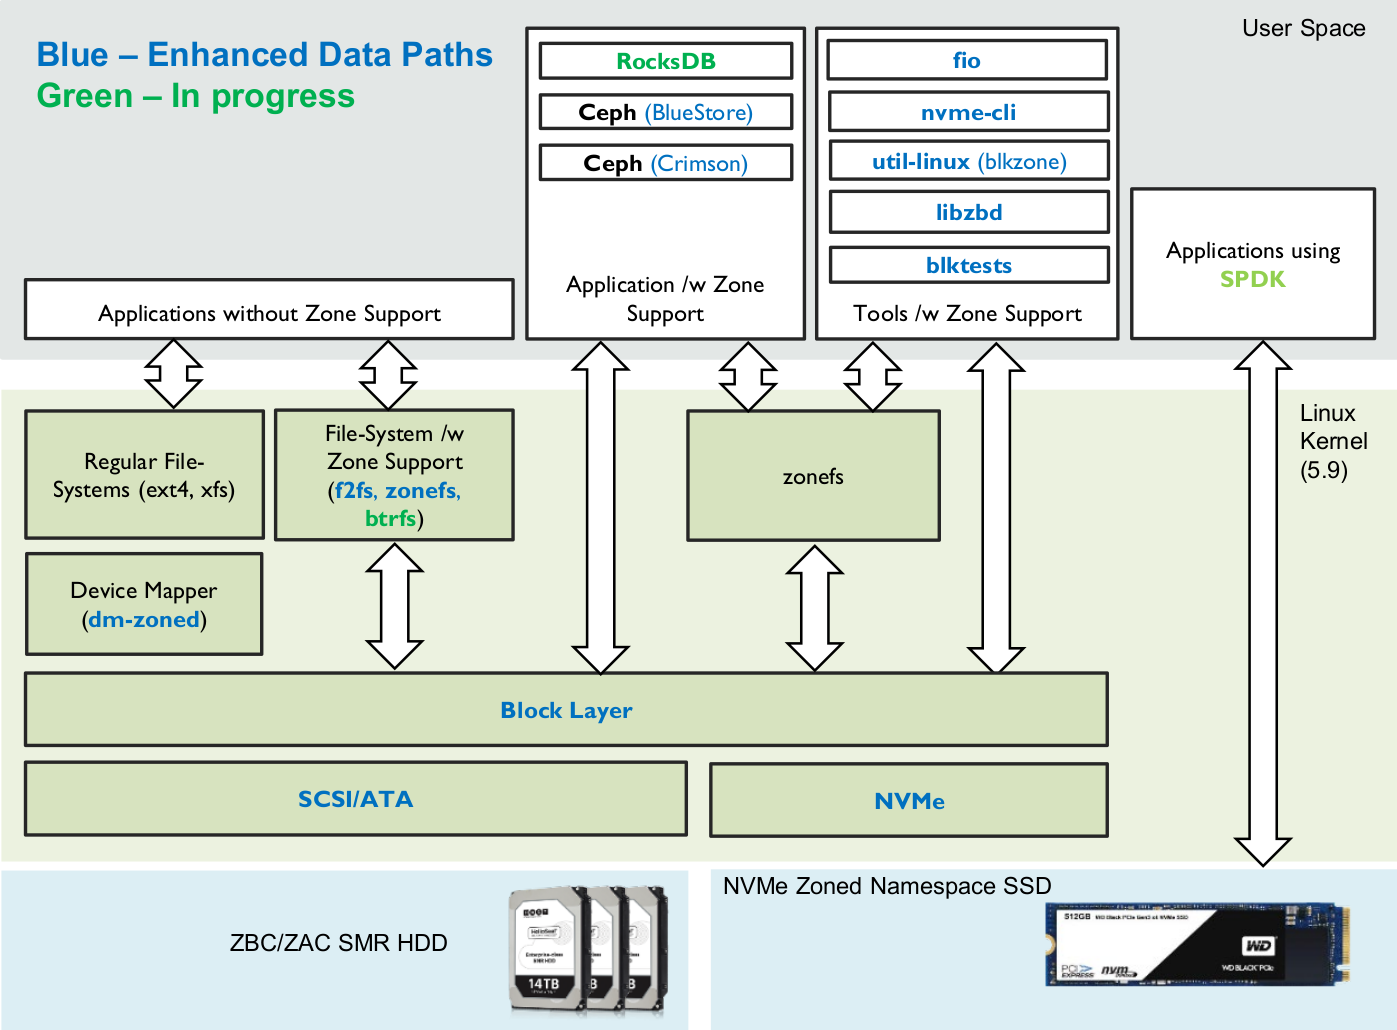
\includegraphics[width=0.5\textwidth]{resources/images/spdk-zns-ssd-landscape.png}
		\captionsetup{justification=centering}
		\caption{Image from Usenix presentation by Matias Bj{\o}rling
			depicting the SPDK landscape\cite{246542}}
		\label{fig:spdk-landscape}
	\end{figure}
\end{center}

\subsection{BPF}

BPF is a complicated and large topic consisting of many different elements. Some
of these elements are very old but have been revised several times over the
years. Problematic is that many of these elements have very similar if not
identical names, yet serve entirely different purposes or are used in an
entirely different context. Many resources have been written on BPF and these
elements, so much so that it would make little sense to try and encapsulate that
in this work.

Instead an overview of resources is provided along with their relative size,
value and age. These resources are categorized into four groups. Each of these
groups is briefly introduced along a graphical representation of all the
different elements. This brief description along with a visual overview should
reduce the confusion when reading about all these similarly named elements.

The categories include \textit{Linux Kernel}, \textit{BPF CO-RE \& BTF},
\textit{libbpf} and \textit{userspace execution / interpretation}. These
categories are chosen as BPF is an inherit part of the Linux Kernel. It consists
of several parts including an ABI, virtual machine and bytecode verifier.

This ties into the second category \textit{BPF CO-RE \& BTF}. Since BPF is
executed within the kernel it can also access datastructures used by the kernel.
This introduces a huge compatibility problem as these datastructures typically
change often with kernel versions. BPF CO-RE and BTF are technologies used to
ensure a BPF program can run regardless of kernel version. Although correctly
using these technologies requires additional programming effort compared to
writing regular BPF programs.

BPF programs typically aren't run directly which is done using syscalls.
Instead, a runtime library is used from which these syscalls are called.
Many of these runtimes exist ranging from large frameworks to small
bootstrapping libraries. Given the intriquisies of these large frameworks they
are not covered in these work. The third category provides resources on these
runtime libraries and is named \textit{libbpf}.

The final category involves the environments in which to execute these BPF
programs. As hinted earlier, the Linux kernel contains a virtual machine that
can execute these programs. However, the Linux kernel is not the only virtual
machine implementation that can execute these. The last category is named
\textit{execution / interpretation}.

The overview of all these resources, their categories, value, length and age
is shown in table \ref{table:bpfresources}. Before continuing with reading the
next section it is advised to at least read all resources with value
\textit{high}.

\begin{table}[h!]
	\caption{BPF resources and their relevance}
	\label{table:bpfresources}
	\centering
	\begin{adjustbox}{width=0.5\textwidth}
		\begin{threeparttable}[]
			\begin{tabular}{lllll}
				\toprule
				\textbf{Resource} & \textbf{Category} & \textbf{Value} &
				\textbf{Length} & \textbf{Age} \\
				\midrule
				\href{https://www.man7.org/linux/man-pages/man2/bpf.2.html}{Linux bpf manpage} &
				Linux Kernel & medium & short & timeless \\
				\href{https://www.kernel.org/doc/Documentation/networking/filter.txt}{BPF kernel documentation} &
				Linux Kernel & low & long & outdated \\
				\href{https://www.kernel.org/doc/html/latest/bpf/btf.html}{Linux BTF documentation} &
				Linux Kernel \& BTF & low & medium & timeless \\
				\href{https://facebookmicrosites.github.io/bpf/blog/2020/02/19/bpf-portability-and-co-re.html}{BPF portability and CO-RE} &
				BPF CO-RE \& BTF & high & medium & relevant \\
				\href{https://nakryiko.com/posts/libbpf-bootstrap/}{BPF applications with libbpf-bootstrap} &
				libbpf - libbpf-bootstrap & high & short & relevant \\
				\href{https://www.oreilly.com/library/view/linux-observability-with/9781492050193/}{Linux Observability with BPF} &
				libbpf - bpf\_load & medium & book & outdated \\
				\href{https://facebookmicrosites.github.io/bpf/blog/2020/02/19/bpf-portability-and-co-re.html}{Cilium BPF + XDP reference guide} &
				libbpf & high & long & relevant \\
				\href{https://facebookmicrosites.github.io/bpf/blog/2020/02/20/bcc-to-libbpf-howto-guide.html}{BCC to libbpf conversion} &
				libbpf & low & long & relevant \\
				\href{https://github.com/iovisor/ubpf}{uBPF} &
				execution / interpretation & medium & short & relevant \\
				\href{https://github.com/generic-ebpf/generic-ebpf}{generic-ebpf} &
				execution / interpretation & medium & short & relevant \\
				\bottomrule
			\end{tabular}
			\begin{tablenotes}[para,flushleft]
				\centering List of resources on BPF and its various elements.
			\end{tablenotes}
		\end{threeparttable}
	\end{adjustbox}
\end{table}

From these references it should be clear that BPF has been around for a long
time. Nevertheless, it is continuing to see improvements and new additions
including the prominent eBPF or the more recent sleepable BPF
programs \cite{bpf-features}.

\subsubsection{BPF Landscape}

This section serves as a detailed explanation for
figure \ref{fig:bpf-landscape}.

Initially this figure might appear quite complex. therefore, it is important to
break it down in a step by step manner. Effectively, the figure shows two
primary types of relationships. First is a chain of dependencies that is
irrelevant to the order of steps in which an example BPF program is compiled and
executed, these are shown using bold white arrows. Secondly, is a step by step
execution flow to compile and execute a BPF program, these are shown using thin
arrows with various colors and patterns. A striped arrow pattern is used to
indicate that the use of this dependency is optional. While the colored arrows
are used to show alternatives to the basic execution of BPF programs
inside the Linux kernel. Finally, all thin arrows are numbered to show the
absolute order of individual steps.

The figure also highlights a clear separation of userspace and kernel space
components. As well as indicating to which particular stage a technology
belongs. Finally, for each kernel space component the figure highlights the
kernel version at which this component was introduced. A short legend for
different elements is shown in figure \ref{fig:bpf-landscape-legend}.

\begin{center}
	\begin{figure}[H]
		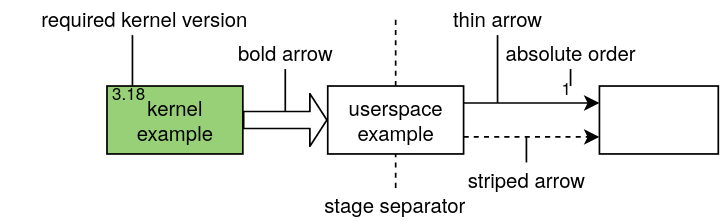
\includegraphics[width=0.5\textwidth]{resources/images/bpf-landscape-legend.png}
		\captionsetup{justification=centering}
		\caption{Legend for the BPF landscape figure}
		\label{fig:bpf-landscape-legend}
	\end{figure}
\end{center}

The following explanation describes the step by step process of executing a BPF
program. At each step the use of optional dependencies or alternative execution
environments is discussed. Running a BPF program start by compiling the source
code using Clang, the use of Clang is recommended as it supports
generating BPF bytecode directly. With the bytecode generated we now need to
compile a runtime program that facilitates loading this bytecode and submitting
it to an execution environment. The compilation of the BPF bytecode and runtime
program are decoupled as BPF bytecode is only loaded at runtime as a function
argument.

From this diagram it might be apparent that compiling and running BPF programs
is non-trivial. One of the reasons is due to differences between different
kernel versions. As described in references from table \ref{table:bpfresources},
BPF CO-RE helps  alleviate these issues by providing translation mechanisms.
Ensuring BPF CO-RE compatibility starts when compiling the BPF program into
bytecode with clang. This is why LLVM clang is drawn across the border of the
compilation and BPF CO-RE stages. Specifically, Clang can emit BTF relocations
metadata that can be used for translation at runtime.

Normally runtimes that support BPF CO-RE require BTF as dependency. This header
is located in the Linux source, however, since kernel 5.5 a special sysfs file
is also available. This sysfs file is able to generate a \textit{vmlinux.h}
header without kernel sources.

Depending on the runtime this \textit{vmlinux.h} header might be used to
perform the necessary BTF translations. Alternatively the BTF header might be
used directly, typically it can either be found in the kernel headers or in
\textit{/usr/include/linux}.

One particular trap is that Ubuntu based Linux
distributions their \textit{/usr/include/linux} directory will always contain
headers for the regular release kernel, even if the so called \textit{HWE}
kernel is installed. For 18.04 releases this can be particularly problematic as
this directory will now contain headers for 4.15 even if 5.4 is installed and
running.

So using the \textit{libbpf} runtime might still require installing kernel
headers depending on the Linux distribution used. Other runtimes have even
larger requirements such as \textit{bpf\_load}. This is a set of headers and
source files contained in the Linux source until version 5.10, however, these
files are not included in kernel header packages or \textit{/usr/include/linux}.

The number of available runtimes as well as their dependencies is quite a
complicated part of BPF. For simplicity, large standalone runtime frameworks
such as BCC and bpftrace are excluded. In addition, the concept of running BPF
programs solely relying on kernel headers is not discussed.

This results in 3 different runtimes of which every runtime is dependent on
\textit{libbpf} or is \textit{libbpf} itself. Alternatives to \textit{libbpf}
are \textit{libbpf-bootstrap} and \textit{bpf\_load}. Where the first
alternative also depends on \textit{vmlinux.h}.

From these runtimes, the use of \textit{libbpf-bootstrap} makes the most
intuitive sense. This is because the generation of \textit{vmlinux.h} is more
straightfoward than including kernel headers or even the entire Linux kernel
sources. Additionally, \textit{bpf\_load} is no longer available as of the most
recent version of the Linux kernel.

When the runtime is chosen, it can be used to compile a program that will load
and execute a BPF program. The functions available to achieve this depend on
the runtime. Typically the runtimes are compiled independently and linked as
shared or static libraries.

These runtimes will make the necessary syscalls to the Linux kernel under the
hood. However, the Linux kernel performs static verification steps before
actually executing the BPF program inside its virtual machine.

Executing BPF programs inside the Linux kernel might actually not be desirable,
for instance when using a userspace NVMe driver such as SPDK. In these cases
alternative execution environments such as \textit{uBPF} and
\textit{generic-ebpf} are available. These, however, do not rely on overriding
specific kernel syscalls so they have to be explicitly programmed at compile
them as they offer an alternative API.

\onecolumn

\begin{center}
	\begin{figure}[H]
		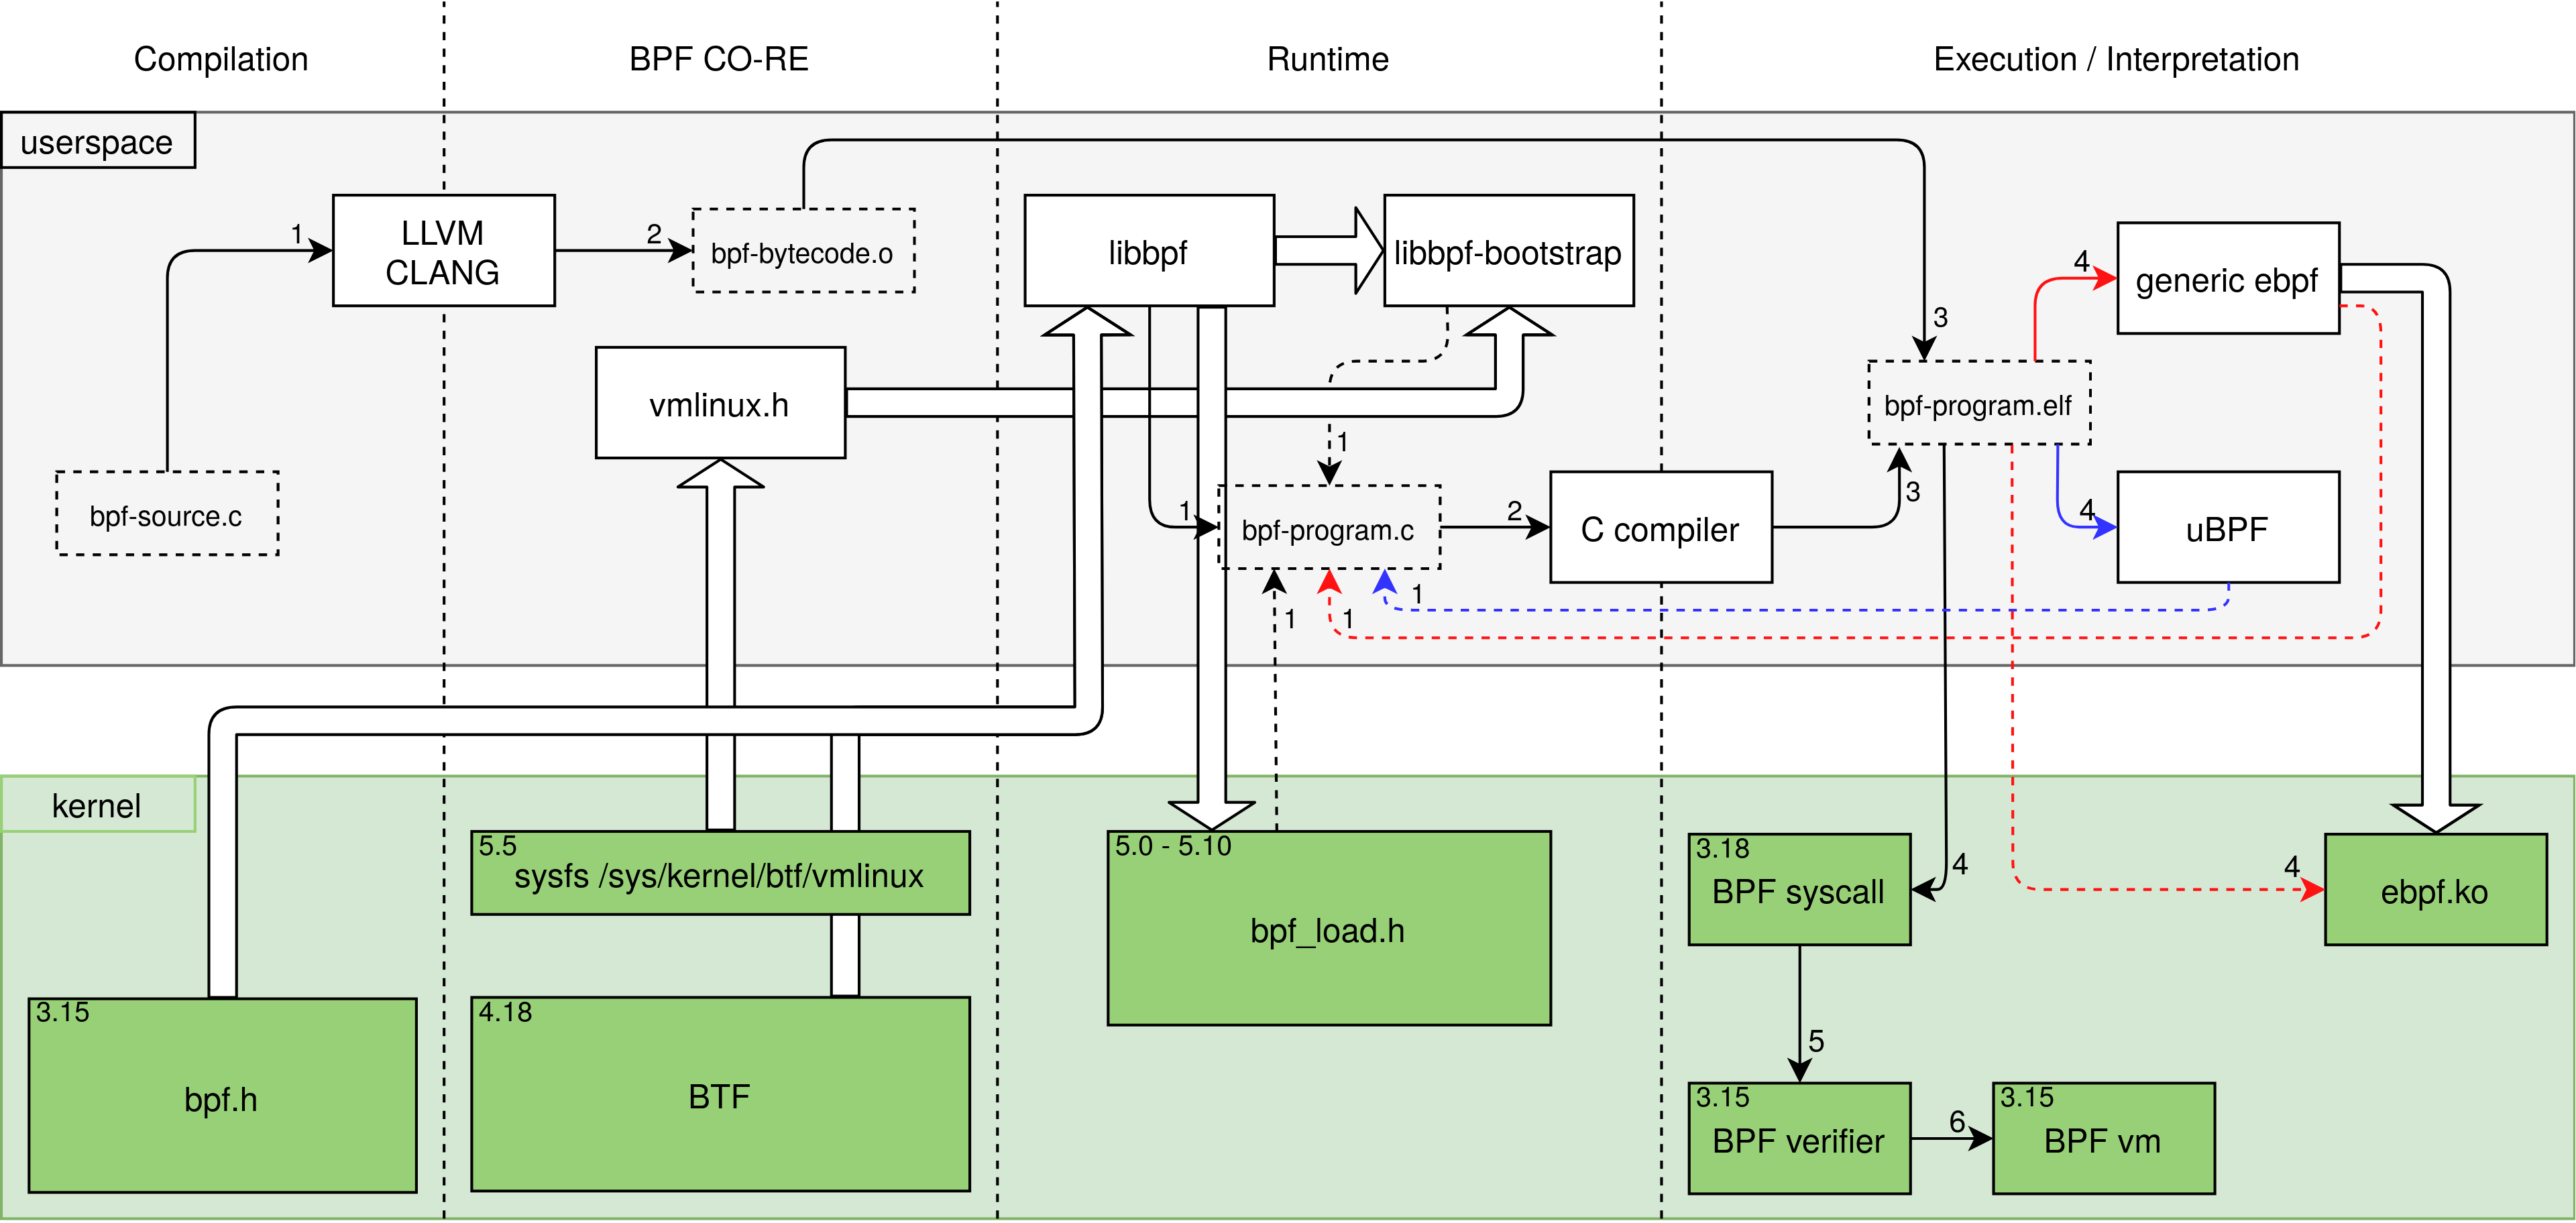
\includegraphics[width=1\textwidth]{resources/images/bpf-landscape.png}
		\captionsetup{justification=centering}
		\caption{Overview of BPF landscape across various stages of use}
		\label{fig:bpf-landscape}
	\end{figure}
\end{center}

\twocolumn

\subsubsection{BPFtool}

A final tool for BPF can be compiled from the Linux source and is called
BPFtool. This binary is what generates the \textit{vmlinux.h} header from
sysfs. However, it can also generate a skeleton header from BPF object files.
This header can be included at compile time preventing loading the object file
from disk at runtime. When used in conjunction with BPF CO-RE these skeleton
headers also allow to modify global variables before the BPF program is run.
The modification of these global variables after compilation is achieved through
BPF relocation instructions.

\section{Design}

The following sections now introduce the design requirements, the implemented
design, the limitations of this design and finally which technologies are not
used in the design and for which reason.

\subsection{Design Requirements}

In this section the design requirements and more optional desired features are
detailed. These requirements try to reason about what is essential to research
CSDs using NVMe ZNS. Desired features try to take this one step further and
reason about the several research questions researcher might have and what that
would require.

Firstly, the design must allow to create and expose interfaces as if a new API
or standard is developed. These could include a new NVMe command set or the
API available to the BPF programs running on the CSD.

Secondly, from the abstraction it must be clear what is being executed on the
host and what is being executed on the CSD. In addition, the data transmitted
over PCIe bus in comparison to the data read or written on the CSD must be clear
from the abstraction.

Lastly, the programs running on the CSD must be able to actually read and write
from a ZNS SSD.

These minimum requirements can be easily extended. Firstly, the design could
automatically monitor the relation of data between host and CSD, generating on
the fly statistics. These statistics can be made to create performance
predictions based on theorized bus and device bandwidth as well as latencies.

Secondly, the design could incorporate functionality for having multiple
compute cores on a single CSD with an accompanying scheduler.

Lastly, the design could introduce tokens or other objects to introduce security
features that ensure CSD programs are only allowed some specific operations.

The essential design requirements are applicable to general CSD research
questions, however, any of the optional features might already lead into a more
specific research question. For this reason it might be better to focus on the
design requirements and leave any optional features to follow up research.

\subsection{Implemented Design}

The final prototype uses a combination of SPDK, uBPF and BPFtool. In this
design SPDK is configured to use the first zoned namespace on a NVMe controller
it can find. Subsequently, this SPDK state is passed to an abstraction which
exposes a hypothetical extension to the NVMe command set.

This abstraction is called \textit{NvmCsd} in this design. As bare prototype it
only exposes two commands. One, to send a BPF program in ELF format, another to
retrieve the return data of the BPF program after it has finished executing. The
interface of these commands is shown in figure \ref{fig:nvm-commands}.

\begin{center}
	\begin{figure}[H]
		\cexternal{resources/c/nvm-commands.c}
		\captionsetup{justification=centering}
		\caption{Interface of two prototype new NVMe commands}
		\label{fig:nvm-commands}
	\end{figure}
\end{center}

The state of SPDK is never used by \textit{NvmCsd} directly only from uBPF. uBPF
provides an environment to run BPF programs in. By default no functions will be
available from within the BPF program but uBPF allows to easily define custom
functions. The prototype design defines four functions that primarily allow to
read from the ZNS SSD and store the data somewhere. Providing the BPF program
a region to store data is essential as uBPF only offers a limited 128 byte stack
space as well as performing thorough bounds checking upon each memory access.
For this prototype a default value of 512K of memory is provided to the BPF
program.

The method to define functions for BPF programs is shown in
figure \ref{fig:bpf-functions}. Notice, how each function is assigned to a
specific number. These numbers will be used for the BPF call instruction that
takes a number as argument. Importantly, these definitions will be defined
in two separate headers, one for use by the BPF program and one for the actual
implementation on the host.

\begin{center}
	\begin{figure}[H]
		\cexternal{resources/c/bpf_functions.c}
		\captionsetup{justification=centering}
		\caption{BPF function definitions for the prototype}
		\label{fig:bpf-functions}
	\end{figure}
\end{center}

uBPF can execute a BPF program by directly reading it in ELF format. This is why
BPFtool is used. This allows to include the BPF program in ELF format as regular
header file.

The prototype performs a few demo operations to illustrate its functionality.
This includes filling the first zone with random value integers. Followed-by,
submitting a BPF program to read the first sector and return the number of
integers above $RAND\_MAX / 2$. If the ZNS SSD from QEMU is used this will
result in 1024 integers being read of which approximately 512 will be above this
predefined value.

\subsubsection{Components}

Effectively, the current prototype consists out of five components.

\subsection{Design Limitations}

There are two primary limitations to the current implementation. Firstly,
currently only one instance of \textit{NvmCsd} can exist at any point in time.
Secondly, several programming limitations apply to BPF programs.

The design limitation in \textit{NvmCsd} arises from how BPF functions are
registered in uBPF. Since these functions are static, a global instance of
\textit{NvmCsd} is referenced from within these functions. Currently, the last
created instance of \textit{NvmCsd} sets this global instance. Any mitigation
to this limitation ties into the second limitation.

Currently, the uBPF library does not support all instructions of BPF. One of the
most important instructions it does not support is the BPF relocation type 1
instruction. One of the situations in which this instruction is emitted is when
using global variables. To ensure a BPF program is runnable by uBPF one
must assert that no \textit{R\_BPF\_64\_64} is present in the \textit{.text}
section. This can be checked using\bashinline{llvm-objdump -r /path/to/bpf.o}.

The combination of these two limitations creates a problem. Intuitively one
would want a global variable in the BPF program that can be initialized
externally before running. By using this variable in the custom defined BPF
functions, \textit{NvmCsd} would be able to determine to which instance these
calls belong even if the functions themselves are static. For this a global
list that maintains all instances of \textit{NvmCsd} can be used.

As example, imagine a hypothetical scenario in which two instances of
\textit{NvmCsd} exist, each assigned its own SPDK state refererring to entirely
different ZNS SSDs. Both of these instances now run a BPF program that calls
several static functions. From the context of these static functions it is now
impossible to determine to which instance of \textit{NvmCSd} and consequently
which ZNS SSD they belong.

% Describe register initialization solution and relevant Github issue.

\subsection{Alternative Technologies}

\section{Future Work}



%\footnotemark[1]. example\ref{term}.
%\footnotetext[1]{test}
%\subsection*{Accelerated Computing Landscape}
%\textit{C++}
%GPUOCelot\cite{tired-manycore-architectures-ocelot}
%\section{LARGER SECTION}
%$\mathcal{O}(N\log N)$
%
%\begin{center}
%	\begin{figure}[H]
%		\bashexternal{resources/bash/inxi.sh}
%		\captionsetup{justification=centering}
%		\caption{Output of inxi showing both CPU and GPU hardware configuration}
%		\label{fig:inxihardware}
%	\end{figure}
%\end{center}

%\cite{Rius1995,Karp1996,parreverse,Adikaram2014}.

%\begin{center}
%	\begin{figure}[H]
%		\cexternal{resources/c/basic.c}
%		\captionsetup{justification=centering}
%		\caption{First basic kernel}
%		\label{fig:base}
%	\end{figure}
%\end{center}

\addcontentsline{toc}{section}{\protect\numberline{}TERMINOLOGY} 
\section*{TERMINOLOGY} \label{term}

This section hopes to define some common terminology as well as clearly detail
how some of these terms are interpreted. Mainly, this section serves to avoid
confusion.

%\begin{tabularx}{\textwidth}{@{}l<{ -}@{\ }X@{}}
%	ZNS & Zoned Namespace \\
%	CSD & Computational Storage Device \\
%	Upstream & When a certain patch or feature has been \\ merged into the main
%		repository of a project. \\
%
%\end{tabularx}

\begin{enumerate}
	\item ZNS - Zoned Namespace
	\item CSD - Computational Storage Device
	\item Upstream - When a certain patch or feature has been merged into the
					 main repository of a project.
	\item GUI - Graphical User Interface
	\item IDE - Integrated Development Environment
	\item Target - A target is something that can be compiled or generated and
					 sometimes executed. Examples include PDFs using LaTeX,
					 binaries or libraries.
	\item Binary   - A binary is a file containing machine instructions that can
					 be directly executed. A compiled C file containing a main
					 method is a binary while a shell script is not. Typically
					 these binaries contain metadata information to aid the
					 underlying operating system in executing them, a common
					 format for this metadata is ELF.
	\item ABI      - Application Binary Interface.
	\item API      - Application Programming Interface.
	\item SCSI     - Small Computer System Interface
	\item ATA      - AT Attachment
	\item ZBC      - (SCSI) Zoned Block Command
	\item ZAC      - (ATA) Zoned ATA Commands
\end{enumerate}

\addcontentsline{toc}{section}{\protect\numberline{}REFERENCES}
\bibliographystyle{IEEEtran}
\phantomsection
\bibliography{bibliography}


%% \begin{center}
% 	\begin{figure}[H]
% 		\includegraphics[width=0.5\textwidth]{resources/mape-k.png}
% 		\captionsetup{justification=centering}
% 		\caption{Diagram of MAPE-K feedback loop \\ CC-BY 4.0$^{0}$}
% 		\label{fig:mapek}
% 	\end{figure}
% \end{center}

% \begin{table}[h!]
% \caption{Platform migrations}
% \label{table:platformmigrations}
% \centering
% \begin{adjustbox}{width=0.5\textwidth}
% \begin{threeparttable}[]
% \begin{tabular}{lll}
% \toprule 
% \textbf{Original platform} & \textbf{New platform} & \textbf{Status} \\
% \midrule
% \href{https://git.openstack.org}{git.openstack.org} &
% \href{https://opendev.org}{opendev.org} & complete \\
% \href{https://review.openstack.org}{review.openstack.org} &
% \href{https://review.opendev.org}{review.opendev.org} & complete \\
% \href{https://launchpad.net}{launchpad.net} &
% \href{https://storyboard.openstack.org/}{storyboard.openstack.org} & ongoing \\
% \bottomrule
% \end{tabular}
% \begin{tablenotes}[para,flushleft]
%      \centering List of platform migrations and their status.
% \end{tablenotes}
% \end{threeparttable}
% \end{adjustbox}
% \end{table}

% \addcontentsline{toc}{section}{\protect\numberline{}Abbreviations}
% \section*{Abbreviations}

% \begin{enumerate}
% 	\item AUAS  - Amsterdam University of Applied Sciences
% 	\item TI    - Technical Informatics
% 	\item ALICE - A Large Ion Collider Experiment
% 	\item RPS   - Resource Provisioning Services
% 	\item API   - Application Programming Interface
% 	\item AQMP  - Advanced Message Queuing Protocol
% 	\item UUID  - Universally unique identifier
% 	\item R\&D  - Research and Development
% 	\item IaaS  - Infrastructure as a Service
% 	\item CERN  - European Organization for Nuclear Research
% 	\item LHC   - Large Hadron Collider
% 	\item PTL   - Project Team Lead(er)
% 	\item REST  - REpresentational State Transfer
% 	\item RFC   - Request For Comments
% 	\item HTTP  - HyperText Transfer Protocol
% 	\item SQL   - Structured Query Language
% 	\item YAML  - YAML Ain't Markup Language
% 	\item EOL   - End Of Life
% 	\item OOM   - Out Of Memory
% 	\item JSON  - JavaScript Object Notation
% 	\item PoC   - Proof of Concept
% 	\item CU    - Compute Unit
% 	\item RAM   - Random Access Memory
% \end{enumerate}

% \onecolumn

% \addcontentsline{toc}{section}{\protect\numberline{}Appendix}
% \section*{\large Appendix}

% \begin{table}[h!]
% \addcontentsline{toc}{subsection}{\protect\numberline{}Watcher collaboration
% resources}
% \caption{Online resources regarding governance \& collaboration for Watcher}
% \label{table:collabresources}
% \centering
% \begin{adjustbox}{width=\textwidth}
% \begin{threeparttable}[]
% \begin{tabular}{ll}
% \toprule 
% \textbf{Source} &\textbf{Content} \\
% \midrule
% https://www.openstack.org/ & Entry into many important other online resources \\
% https://wiki.openstack.org/wiki/Watcher & Watcher entry for many online 
% resources \\
% https://launchpad.net/watcher & Bug tracker for issues of OpenStack components
% such as Watcher \\
% https://storyboard.openstack.org/ & New bug tracker to eventual replace 
% launchdpad \\
% https://review.openstack.org/ & Patch and review system capable of
% verifying patches using unit \& functional tests \\
% https://review.opendev.org/ & Replacement for review.openstack.org introduced
% around May 2019 \\
% https://github.com/openstack/watcher & Repository hosting the Watcher source
% code \\
% https://opendev.org/openstack/watcher & New repository for hosting source code
% introduced in May 2019 \\
% https://governance.openstack.org/ & Information how a set of organizational
% bodies organizes the governance \\
% \bottomrule
% \end{tabular}
% \begin{tablenotes}[para,flushleft]
%      \centering This overview lists all online resources used to analyze how
%      watcher is governed and collaborates.
% \end{tablenotes}
% \end{threeparttable}
% \end{adjustbox}
% \end{table}

% \subsection*{Meeting suggestion email}
% \addcontentsline{toc}{subsection}{\protect\numberline{}Meeting suggestion email}
% \label{appendix:suggestionemail}

% \noindent Hello everyone,

% \noindent We would like to propose reintroducing the meetings after the release
% of \\ Stein. I feel meetings are important as it allows us to discuss what we \\
% want to work on and what problems we are experiencing with regards to \\
% Watcher. A notable example of a topic that I feel we should address is \\
% the deadlock in python 3.7 with unit tests. \\

% \noindent Currently we have a meeting scheduled every week but in different \\ 
% channels at different times, however, the documentation is unclear about \\
% the exact time and channel as the following two web-pages disagree: \\
% https://docs.openstack.org/watcher/latest/contributor/contributing.html \\
% https://wiki.openstack.org/wiki/Watcher \\

% \noindent  I would like to propose a meeting on Wednesday at 08:00 UTC on
% even \\ weeks in \#openstack-meeting-4 as I feel this time work bests for
% our \\ mixed time-zones. \\

% \noindent I look forward to hearing from you. \\

% \noindent Kind Regards, \\
% \noindent Corne Lukken \\

% \subsection*{Watcher Drivers team email}
% \addcontentsline{toc}{subsection}{\protect\numberline{}Watcher Drivers team email}
% \label{appendix:driveremail}

% \noindent Done. \\

% \noindent Have a nice day!  Thanks for contributing on Watcher ! \\

% \noindent Jean-Emile
% \noindent DARTOIS \\

% \noindent \{P\}     PhD Student
% \noindent Cloud Computing \\

% \noindent \{T\}     +33 (0) 2 56 35 8260 \\
% \noindent \{W\}     www.b-com.com

% \noindent \_\_\_\_\_\_\_\_\_\_\_\_\_\_\_\_\_\_\_\_\_\_\_\_\_\_\_\_\_\_\_\_\_\_\_\_\_\_\_\_\\
% \noindent De : info@dantalion.nl <info@dantalion.nl> \\
% \noindent Envoyé : jeudi 13 juin 2019 10:23 \\
% \noindent À : Jean-Émile DARTOIS \\
% \noindent Objet : Re: The Watcher Drivers team seems poorly maintained \\

% \noindent Hello, \\

% \noindent Current PTL is Licanwei if you can make him administrator than we \\
% have regained control that would be much appreciated. \\

% \noindent Kind regards, \\
% \noindent Corne Lukken (Dantali0n) \\

% \noindent On 6/13/19 10:00 AM, Jean-Émile DARTOIS wrote: \\
% \noindent > Hello, \\
% \noindent > \\
% \noindent > Sorry, I'm not involved anymore in Watcher. I added you as an \\
% approved member. Who is the current PTL? I can make him administrator. \\
% \noindent > \\
% \noindent > Best regards, \\
% \noindent > \\
% \noindent > \\
% \noindent > Jean-Emile \\
% \noindent > DARTOIS \\
% \noindent > \\
% \noindent > \{P\}     PhD Student \\
% \noindent > Cloud Computing \\
% \noindent > \\
% \noindent > \{T\}     +33 (0) 2 56 35 8260 \\
% \noindent > \{W\}     www.b-com.com \\
% \noindent > \\
% \noindent > \_\_\_\_\_\_\_\_\_\_\_\_\_\_\_\_\_\_\_\_\_\_\_\_\_\_\_\_\_\_\_\_\_\_\_\_\_\_\_\_\\
% \noindent > De : bounces@canonical.com <bounces@canonical.com> de la part de \\
% Dantali0n < info@dantalion.nl> \\
% \noindent > Envoyé : jeudi 13 juin 2019 09:18 \\
% \noindent > À : Jean-Émile DARTOIS \\
% \noindent > Objet : The Watcher Drivers team seems poorly maintained \\
% \noindent > \\
% \noindent > Hello, \\
% \noindent > \\
% \noindent > It seems like the administrators in the Watcher Drivers team have \\
% not be \\
% \noindent > contributing for a long time. I and several others have requested \\
% \noindent > membership months ago without a response. \\
% \noindent > \\
% \noindent > I was hoping you could make  me or Licanwei administrator so we can \\
% \noindent > regain control over the managed of this team. \\
% \noindent > \\
% \noindent > Kind regards, \\
% \noindent > Dantali0n \\
% \noindent > --\\
% \noindent > This message was sent from Launchpad by \\
% \noindent > Dantali0n (https://launchpad.net/~dantalion) \\
% \noindent > using the "Contact this team's admins" link on the Watcher Drivers\\
% team page \\
% \noindent > (https://launchpad.net/~watcher-drivers). \\
% \noindent > For more information see \\
% \noindent > https://help.launchpad.net/YourAccount/ContactingPeople \\

\end{document}